\documentclass{acm_proc_10ptArticle-sp}
\usepackage[T1]{fontenc}

\begin{document}

\title{Final Assignment - Social Web}

\numberofauthors{3}
\author{
%
% The command \alignauthor (no curly braces needed) should
% precede each author name, affiliation/snail-mail address and
% e-mail address. Additionally, tag each line of
% affiliation/address with \affaddr, and tag the
%% e-mail address with \email.
\alignauthor Arthur-Ervin Avramiea\\
       \affaddr{2517642}\\
       \email{a.e.avramiea@student.vu.nl}
\alignauthor Mihnea Dobrescu-Balaur\\
	\affaddr{2549278}\\
	\email{mihnea@linux.com}
\alignauthor Zilvinas Kucinskas\\
	\affaddr{2547940}\\
        \email{zil.kucinskas@gmail.com}
}

\date{28 March 2014}
\maketitle

\section{Introduction}

With the rise in popularity of the Web, everybody around the world produces content, from local bloggers to global news agencies. This means that the online medium is now full of content, and that is great. The Web embodies diversity and pluralism in opinions, making sure that anybody can find useful content. However, with this much content available, it can be difficult for people to keep track of the items that interest them the most. And because of the decentralised nature of the Web, it can be difficult to find relevant articles.

In order to solve these problems, websites started providing RSS\footnote{http://en.wikipedia.org/wiki/RSS} feeds and more advanced users have started following them. There are even online aggregators, like the recently closed Google Reader\footnote{http://www.google.com/reader/about/}, in which an user could add multiple RSS feeds that he or she is interested in, and then the website will keep track of new articles and display them in managed lists.

The problem with RSS and aggregators like Google Reader is that they are not so user friendly, having a dense interface, similar to a full webmail inbox. Also, they display the articles in a plain way, with lots of text. This all adds up to an overload of information to the user. More recent applications, like Feedly\footnote{http://feedly.com/} and Flipboard\footnote{https://flipboard.com/}, have taken a fresh approach of the problem. They create rich, magazine-like layouts for the articles, and they also help with content discovery, having predefined and curated “feeds” that the users can subscribe to.

We believe that we can take this idea a step further, and create a rich visual timeline, in which the media content (images and videos) take precedence over the text, removing everything but the headline. This timeline helps the users quickly get up to speed with the latest events and news from around the world, and when they find an article that is interesting, they can read it from the original source, with the original layout, in just one click.

Since there is no such thing as one size fits all, our application allows users to select what regions they are interested in, as well as what domains. So, for example, one user might be interested in Politics around the US, while another user might be interested in Tech news from Asia. Personalising a timeline is easy, and a user can store multiple timelines on his or her account.

\section{Structured data}

Our application has to include articles from all over the world, on all possible topics, and to cover this demand we decided to use, first and foremost, the RSS feeds of the main news agencies in the world. Wikipedia provides a list\footnote{http://en.wikipedia.org/wiki/List\_of\_news\_agencies/} of them, grouped by country. Besides news agencies, we also include information from prominent newsletters like the New York Times\footnote{http://www.nytimes.com/} and online publications like The Verge\footnote{http://www.theverge.com}.

Besides XML data (via RSS), we also use the Twitter API in order to get JSON data of the tweets related to any given article.

To enrich the user’s visual experience, besides the media from the original article, we use the Bing search API to find relevant images and videos, that we then later embed in the rendered story.

All the mentioned data sources and others (detailed in the Analysis section) get mixed in a pipeline that builds a JSON object representing the visual summary of the story that we want to render for the user. Then, using Web technologies we fetch the corresponding JSON files in the frontend application and render them, building the timeline.

\section{Data analysis}

In order to give the user an approximation about the impact of the story they are skimming, we use Sentiment140\footnote{http://www.sentiment140.com/} to perform sentiment analysis on the tweets that we found for that story. Since location is important for our application and for our users, we cluster the sentiment results by region. Figuring out where do the tweet authors live exactly is not trivial, since the majority of tweets does not contain location information. To solve this problem, we rely on the information that users share on their profile page. However, since that data is not structured at all, we have to reason about its text value and decide what region it represents. We do this using the Google Geocoding API\footnote{https://developers.google.com/maps/documentation/geocoding/}. 

\section{Zilvinas Kucinskas individual part - sentiment analysis and visualization}

\subsection{Rationale}

Our application not only provides information about hot topics, but also analyzes Twitter posts with each topic. It uses Twitter API to get tweets to each topic. It analyses those tweets using Sentiment140\footnote{http://www.sentiment140.com/} analysis. Some other services use simple keyword based approach to analyse the tweets, but this one uses classifiers built from machine learning algorithms. It can provide both the aggregated sentiments or assesment of an individual tweet. Aggregated information is provided directly on the site using pie diagram, and it is possible to query the service to get data in JSON format. Our application splits tweets by country and provides visualisation using jVectorMap\footnote{http://jvectormap.com/}. This API provides capabilities to generate custom maps or use existing ones. We use world map to provide visualisation of sentiments.

The main rationale behind this feature is providing users with approximation of the impact article gives user's globally. There is three variants of different opinions - positive, negative and neutral. Everytime application is refreshed - new tweets are gathered for each separate article and sentiment analysis is provided. 

According to Wikipedia\footnote{http://en.wikipedia.org/wiki/Data\_visualization}, the main purpose of data visualization is to communicate information. Based on article "\textbf{Why is data visualization so hot?}" \footnote{http://blog.visual.ly/why-is-data-visualization-so-hot/}, humans are able to interpret information way better if they see it visually, because huge amount of data can be transmitted to the brains through the optic nerve. Usually it's hard to understand the data looking only to numbers, but using data visualisation it is possible to see patterns and trends in the data way easier and faster \cite{kaidi}.

In my opinion, every text human reads could provide some impact on him, he may feel angry, scared, astonished, excited, neutral and so on. Usually, the more followers user has, the more it is influential to others. Sentiment analysis and visualisation feature provides our application users the opportunity to compare their sentiments to the ones in the Twitter social network. By splitting sentiments by country, we provide them the opportunity to find some patterns in the sentiment world map. Because each country has separate traditions and culture, people from different countriens feel differently about same topics. For example, occupation in Crimea is a really hot topic right now. By analysing sentiments, we were able to see that Russia has a positive sentiment regarding Crimea and for example France has more negative sentiment about it. So by having this information it is possible to make assumptions that Russia wants to occupy Crimea, and russian media is supporting it and that media from EU, France is against Crimea occupation. This can be shown in the Appendix figure \ref{screenshot:crimea}.

\subsection{Motivation}

Our application is oriented to people, who is interested in reading news articles, for users, who is keen to know what is happening around the world or in different domains of knowledge. By providing only pictures, videos and headline of an article, it is far more easier to search content to read. People can skim pages really fast and select which articles they want to read. They can also personalize their content by specifying which domain or regions he is interested in, also he has an opportunity to have several timelines. By clicking on specific article user gets redirected straight to the article in some online media source.

\subsection{Scoping}

Besides nice features our application also has some limitations. For example pictures and videos extracted from Bing could not always reflect the article, but we believe at least images and videos extracted directly from each online media source article is accurate. For example, there is a screenshot of an article in our application in this report Appendix figure \ref{screenshot:limitation}, which demonstrates this limitation. Also sentiment analysis could not be completely accurate. For example, tweets containing sarcasm can be evaluated completely opposite from it's initial sentiment. And almost always more than 50 percent tweets are evaluated as neutral. This is also a limitation, because variance between positive and negative sentiments is not so obvious.

\subsection{Evaluation}

Evaluation is really important thing in application growth and development. As applications need to be as much friendly and attractive for users, they need to change and adapt over time. First thing would be to look at the users, which are coming back and compare them to new users. Percentage of coming back user would be a good statistic of successfull application overall. This could be easily done by using Google Analytics\footnote{https://www.google.com/analytics}.

Also it would be nice to gather user's preferences and which articles he chooses to look at. It could be possible to analyze gathered data and make a list of most popular articles, and not so popular ones. By having this kind of information it would be possible to look at why people choose on article over another. It could be related with sentiments. It could be possible see if there are any patterns on sentiment analysis, which drives users to see one article over another.

\subsection{Future work}

How would you improve and further develop your application design if time  and efforts would permit?





% The following two commands are all you need in the
% initial runs of your .tex file to
% produce the bibliography for the citations in your paper.
\bibliographystyle{abbrv}
\bibliography{final}

\newpage

%Appendix A
\onecolumn
\section{Appendix}

\ref{screenshot:reader}
\begin{figure}[H]
  \centering
  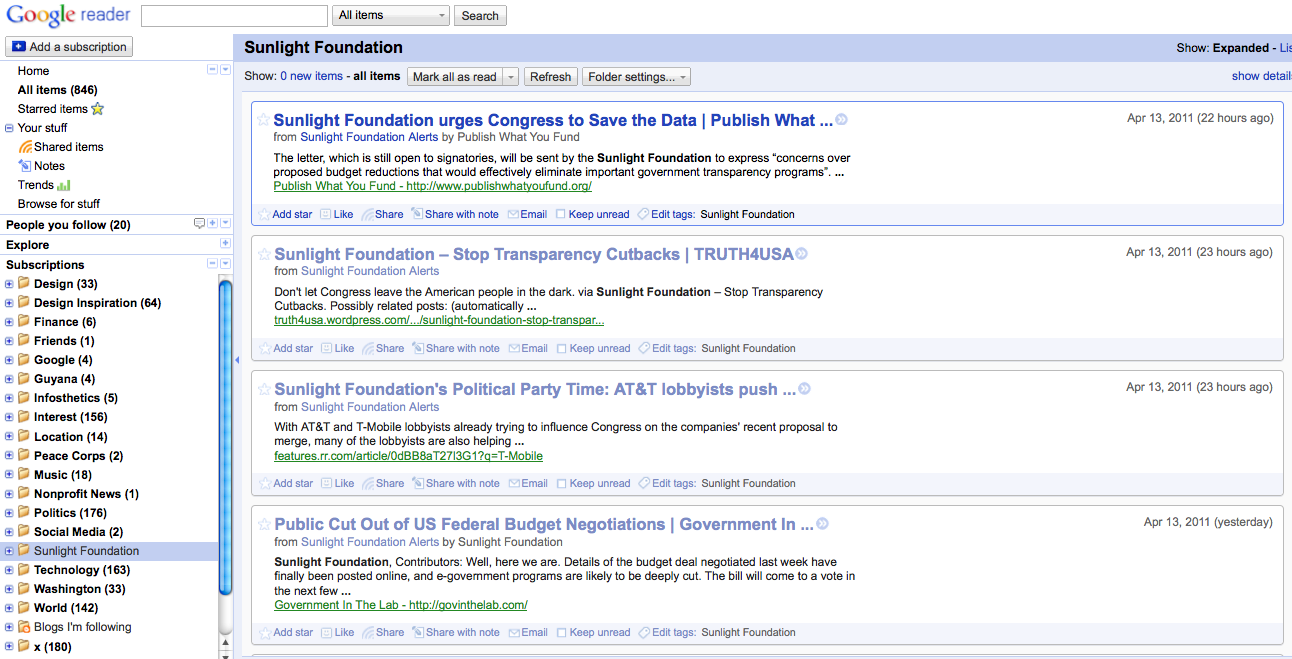
\includegraphics[width=0.9\linewidth]{img/Google-Reader.png}
  \caption{Google Reader screenshot}
  \label{screenshot:reader}
\end{figure}

\ref{screenshot:flipboard}
\begin{figure}[H]
  \centering
  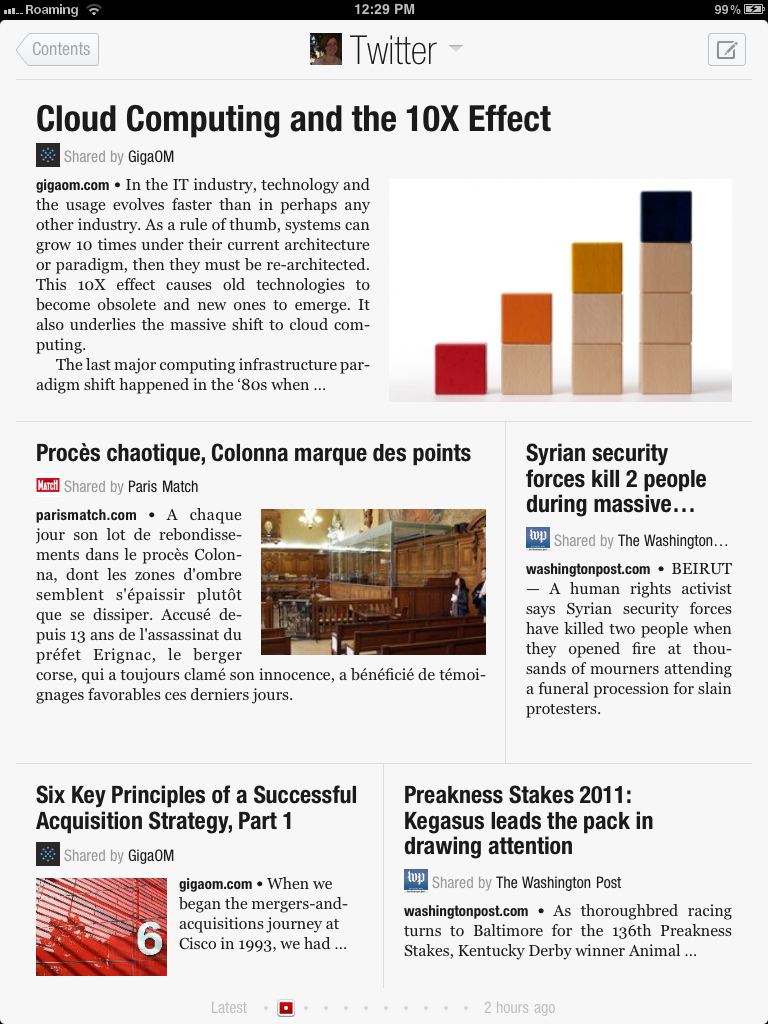
\includegraphics[width=0.9\linewidth]{img/flipboard-screenshot.png}
  \caption{Flipboard screenshot}
  \label{screenshot:flipboard}
\end{figure}

\ref{screenshot:timeline}
\begin{figure}[H]
  \centering
  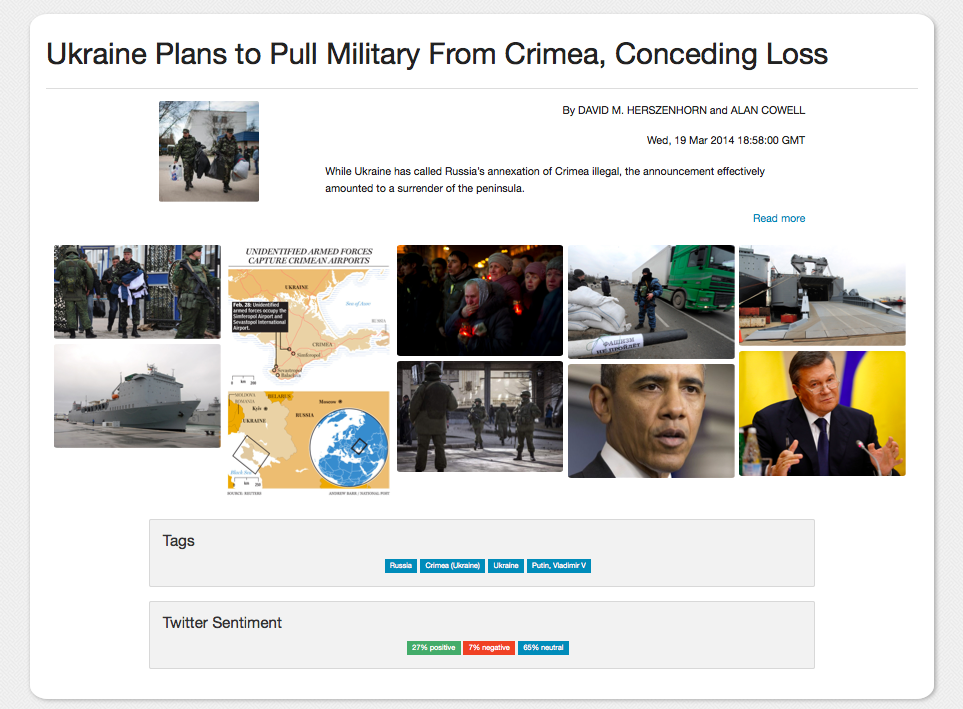
\includegraphics[width=0.9\linewidth]{img/timeline-item.png}
  \caption{Timeline item in our application}
  \label{screenshot:timeline}
\end{figure}

\ref{screenshot:coverage}
\begin{figure}[H]
  \centering
  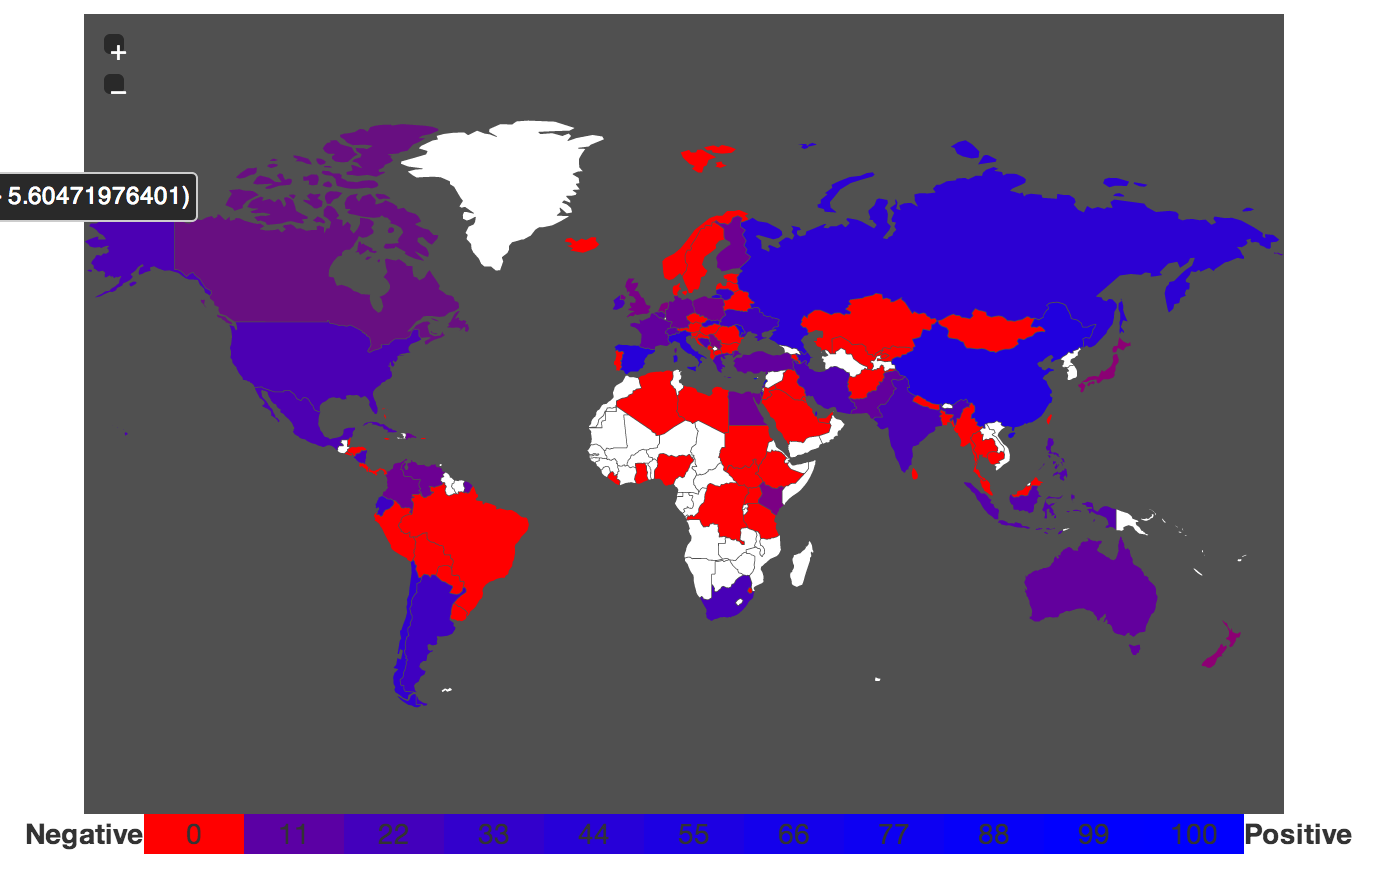
\includegraphics[width=0.9\linewidth]{img/media-coverage-polynomial.png}
  \caption{Media coverage visualization (polynomial)}
  \label{screenshot:coverage}
\end{figure}

\ref{screenshot:crimea}
\begin{figure}[H]
  \centering
  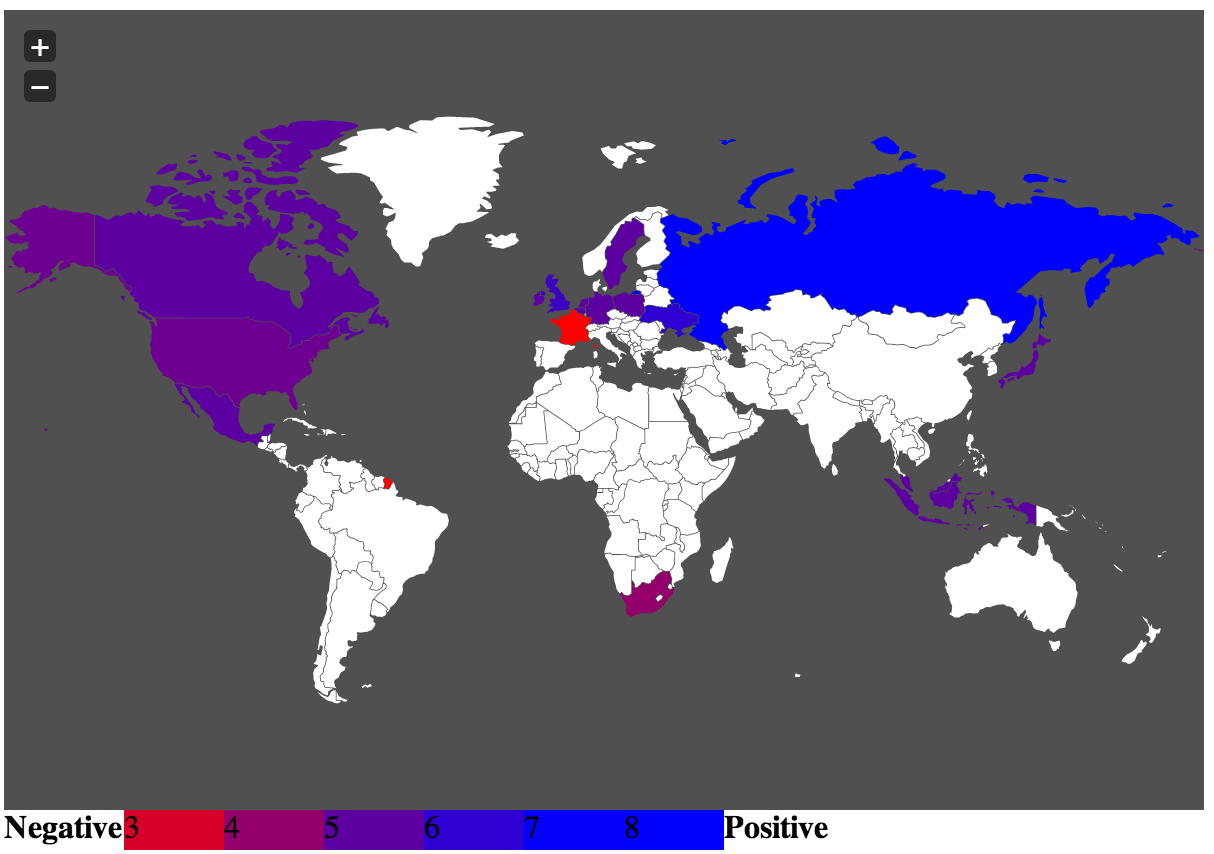
\includegraphics[width=0.9\linewidth]{img/crimea.png}
  \caption{Sentiment analysis about crimea topics}
  \label{screenshot:crimea}
\end{figure}

\ref{screenshot:limitation}
\begin{figure}[H]
  \centering
  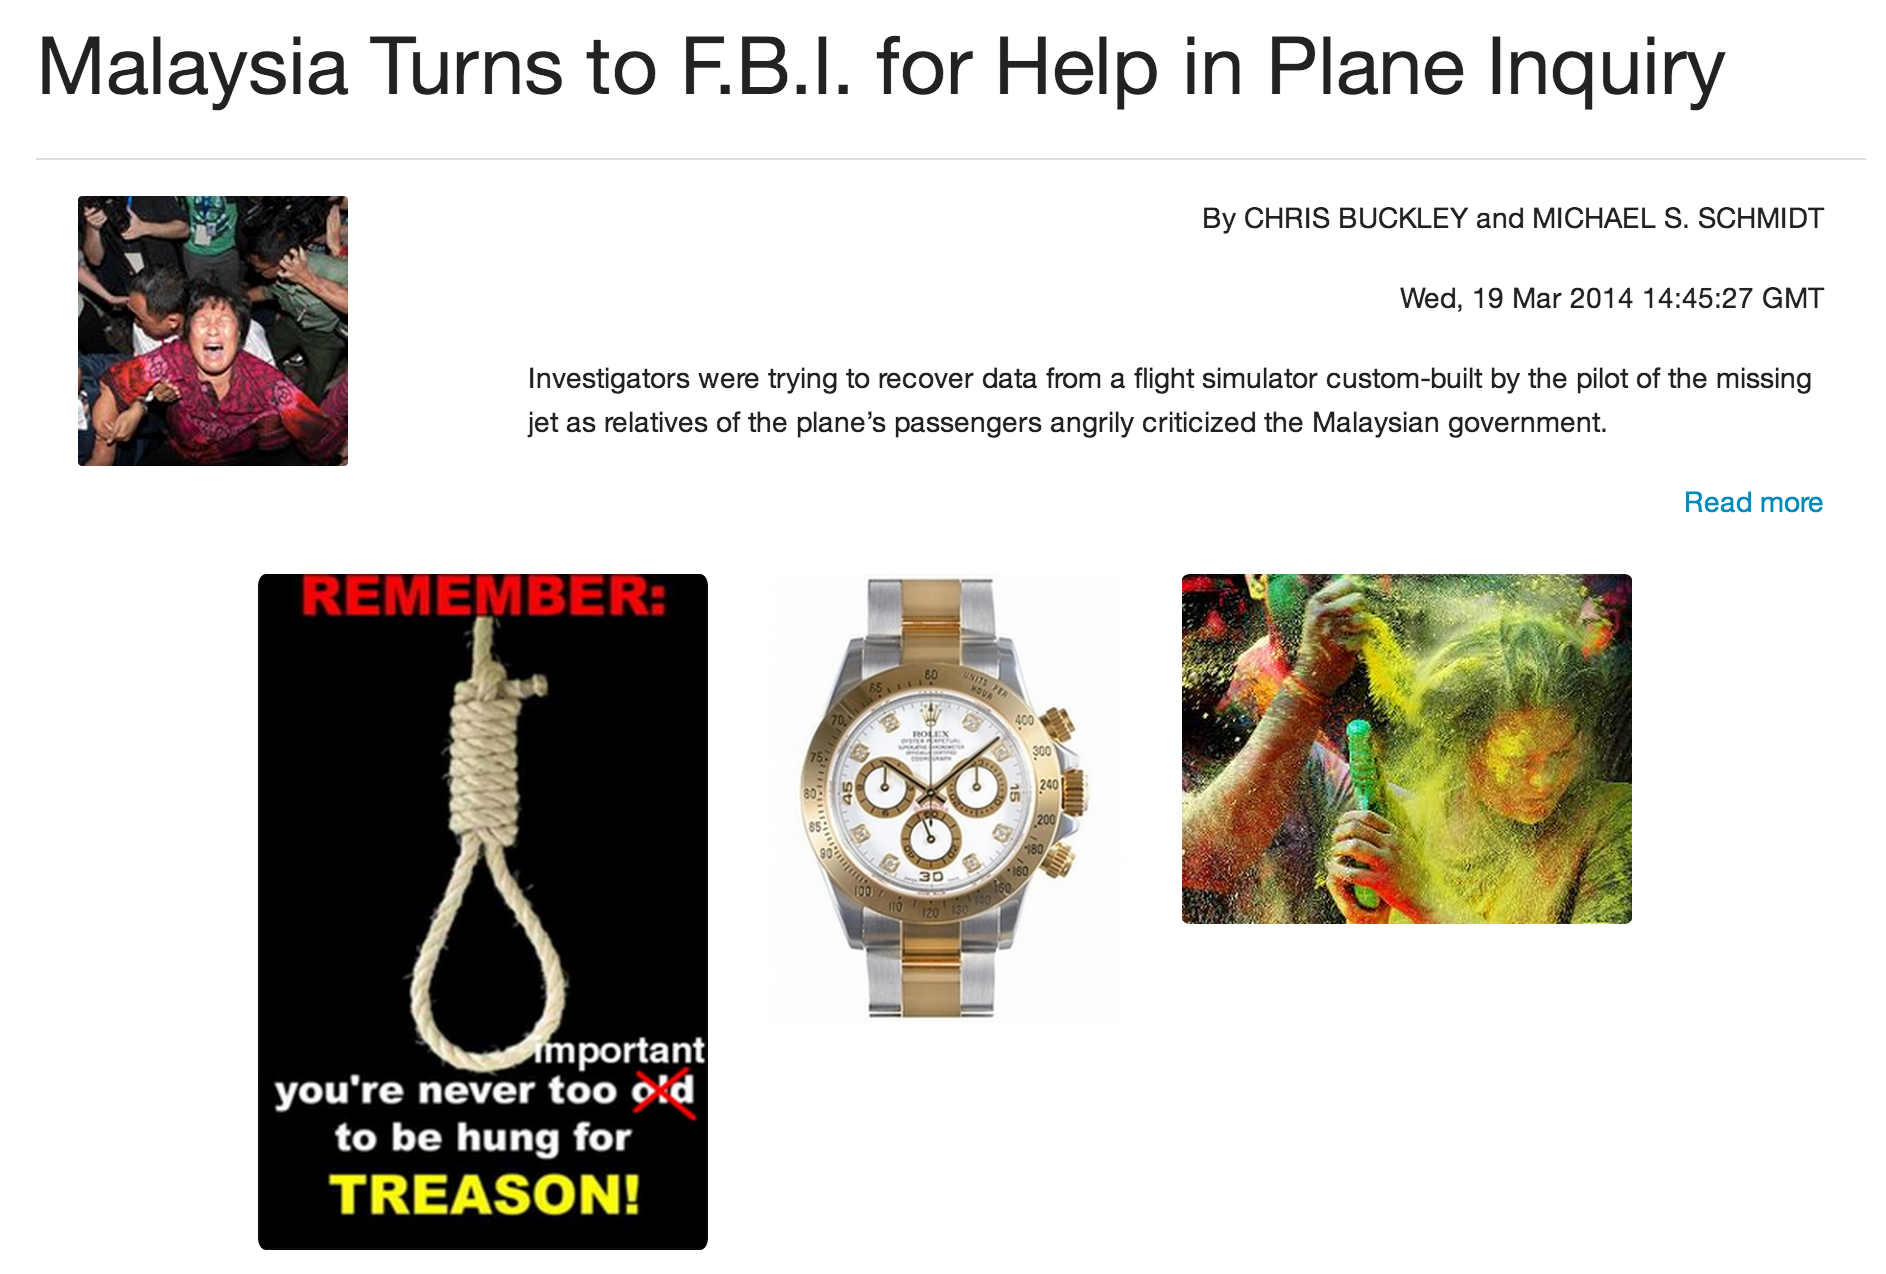
\includegraphics[width=0.9\linewidth]{img/limitation-ZK.png}
  \caption{Screenshot demonstrating scenario with photos from Bing, which are off topic}
  \label{screenshot:limitation}
\end{figure}



% ***********************************************************************
%                           SOME USEFUL EXAMPLES

% Footnote && Caption
% "\textbf{Where in the World Are the Hottest Social Networking Countries?}"
% \footnote{http://www.emarketer.com/Article/Where-World-Hottest-Social-Networking-Countries/1008870}
% \textit{emarketer}

%CITATION
%\citeA{mccombs1972agenda}
% \cite{wanta2004agenda}

% UNFORMATTED CODE EXAMPLE
% \begin{verbatim}
%  {
%     "text": "Russia's 25,000-troop...",
%     "urls": [
%         {
%             "url": "http://rt.com/news/r...",
%             "country_code": "RU"
%         }
%     ],
%     "country_code": "SK"
% }
% \end{verbatim}

% FIGURES
% \ref{screenshot:sentimentmap}
% \begin{figure}[H]
% 	\centering
% 	\includegraphics[width=0.9\linewidth]{crimea_sentiment.png}
% 	\caption{Sentiment analysis}
% 	\label{fig:sentimentmap}
% \end{figure}


\end{document}